%% requires the following packages
%% \usepackage{xspace}
%% \usepackage{caption,subfig,epsfig}
%% \usepackage{amssymb,amsmath}

\newcommand*{\ifb}{fb$^{-1}$\xspace}
\newcommand*{\inbs}{nb$^{-1}$/s\xspace}
\newcommand*{\smhh}{SM $HH$\xspace}
\newcommand*{\bbbb}{\ensuremath{b\bar{b}b\bar{b}}\xspace}
\newcommand*{\bb}{\ensuremath{b\bar{b}}\xspace}
\newcommand*{\ttbar}{\ensuremath{t\bar{t}}\xspace}
\newcommand*{\hh}{\ensuremath{HH}\xspace}
\newcommand*{\bjet}{$b$-jet\xspace}
\newcommand*{\bjets}{$b$-jets\xspace}
\newcommand*{\btag}{$b$-tag\xspace}
\newcommand*{\btags}{$b$-tags\xspace}
\newcommand*{\btagging}{$b$-tagging\xspace}
\newcommand*{\btagged}{$b$-tagged\xspace}
\newcommand*{\mhh}{\ensuremath{m_{HH}}\xspace}
\newcommand*{\mh}{\ensuremath{m_{H}}\xspace}
\newcommand*{\pt}{\ensuremath{p_T}\xspace}

\section{$HH\to\,$\bbbb: Status and Perspectives}
\label{sec:HH4b}

The plurality of \hh events decay via the \bbbb channel ensuring searches in the four \bjet final state dominant sensitivity above some value of \mhh.
Since the start of Run-2, much of the experimental effort has been in lowering this sensitivity limit by loosening kinematic cuts
and modeling the substantially increased background acceptance as illustrated in Figure \ref{fig:2015vs20184b}.
Unfortunately, most of the impact of modifications to the Higgs cubic coupling to the \hh cross section is near the $2\times$\mh threshold.
In this phase space the irreducible multi-\bjet background is on the order of 300$\,$fb with signal efficiencies around 1\%.

\begin{figure}
  \begin{center}
    \subfloat[2015 Analysis \cite{EXOT-2015-11}
      \newline $\approx 15$ events per \ifb
      \newline $\approx 30\%$ statistical uncertainty at peak]{
      \includegraphics[height=4.6cm]{./figures/HH4b/m4j_SR_2015.pdf}}\hfill
    \subfloat[2018 Analysis \cite{Aaboud:2018knk,Bryant:2644551}%% \bf{UPDATE WHEN PAPER IS OUT}
      \newline $\approx 300$ events per \ifb
      \newline $\approx  3\%$ statistical uncertainty at peak]{
      \includegraphics[height=4.4cm]{./figures/HH4b/data_hh_v_logy_2016.pdf}}
    \caption{Loosened kinematic cuts in the most recent ATLAS search increased the background acceptance by a factor of twenty relative to the restricted phase space probed in the first Run-2 result.
      The statistical uncertainty in the peak of the background is now at the percent level. Note the change in y-axis range in the ratio plots.}
  \label{fig:2015vs20184b}
  \end{center}
\end{figure}

Maximising the physics potential of the \bbbb channel thus requires precision modeling of complex backgrounds without reliable simulation
and the ability to trigger on events with multiple, generically soft \bjets. In section \ref{sec:current4b} we introduce the current
approaches to these challenges. Section \ref{sec:limitations4b} outlines the limitations of the existing methods. Section \ref{sec:improvements4b}
lays out possible paths forward where there is clear room for improvement and opportunities for innovation. 

\subsection{Current Strategies}
\label{sec:current4b}

%% ATLAS: 2b->4b extrapolation
The approach taken by the ATLAS collaboration since the beginning has been to model high \bjet multiplicity events with low \bjet multiplicity events.
This procedure relies on the assumption that the ratio of multijet production matrix elements with different \bjet multiplicities doesn't change sharply in the phase space with dijets near the Higgs mass.
Simply by measuring this ratio and the kinematic sculpting from \btagging, one can reweight low \bjet multiplicity events to look like high \bjet multiplicity events.
These reweighting factors should apply equally well across a broad range of phase space with different dijet masses, in particular they should apply for events with two dijets near the Higgs mass. 
ATLAS explicitly checks this assumption by defining orthogonal kinematic selections and using the reweighting factors derived in one to model the others. 

%% CMS: Functional fit for resonance searches \cite{Sirunyan:2018zkk} and hemisphere mixing for non resonant HH search \cite{CMS-PAS-HIG-17-017}.
The CMS collaboration has implemented several different strategies;
their most recent search for resonant \hh production performs a direct functional fit to the \mhh spectrum in the signal region
after validating the background function in kinematic and reduced \btag multiplicity control regions \cite{Sirunyan:2018zkk}.

For their non-resonant search CMS developed a novel 'hemisphere mixing' technique whereby fake events are generated by mixing and matching dijet systems from separate events \cite{CMS-PAS-HIG-17-017}.
The matching algorithm is designed to create physically reasonable fake events with the same kinematic structure as the background process while washing out the correlated structure of the signal process.
The fake events are then used as the background sample in the training of a single Boosted Decision Tree (BDT) classifier to separate signal from background.
A search is then performed for an excess in the tail of the BDT output distribution.

%%Trigger: L1 multijet triggers ~3kHz, HLT b-tag triggers ~40Hz in 2016/2017. (John’s slides) ATLAS measures trigger object level efficiencies and combines them to estimate event level efficiency. See my thesis chapter 9 for detailed explanation of this method.
Both ATLAS and CMS rely on multijet triggers at L1 with online \btagging applied in the HLT to a subset of the online jets.
The primary triggers for CMS require four jets and three online \btags with \pt thresholds between 30 and 90\,GeV.
The primary trigger for ATLAS requires four jets with $\pt>35\,$GeV where at least two are \btagged online at the 60\% working point.
At L1 these trigger items fired at approximately 3\,kHz requiring significant HLT resources for the online \btagging which reduced trigger rates to roughly 40\,Hz. 

\subsection{Limitations of Current Strategies}
\label{sec:limitations4b}

While ATLAS focused on providing a unified analysis strategy for all $\hh\rightarrow\bbbb$ searches,
CMS experimented with independent strategies for low, intermediate and high mass resonances and non-resonant production.
Given the relatively different experimental challenges and event topologies of these regimes, it is not a priori obvious if the unified or divide and conquer approaches will provide better results.
It is certainly useful to now be able to evaluate the limitations of a broad set of approaches. 

%%ATLAS: statistically limited validation technique, focus is on 1D model of final mHH discriminant in single Signal Region; less optimal than high dimensional model/MVA.
%%Iterative reweighting handles correlations in 2b->4b extrapolation. Requires triggers with no more than 2 online b-tags.
The ATLAS and CMS approaches all suffer from statistically limited validation regions.
The assumptions that go into generating a background model from data should not be assumed to hold to a higher degree of precision than can be tested outside of the signal region.
Such uncertainties are difficult to quantitatively assess, particularly when they have nontrivial effects on distributions beyond their normalization.

The recent ATLAS result \cite{Aaboud:2018knk,Bryant:2644551} attempted to address this by deriving the background model twice
using orthogonal kinematic selections and using resulting the variation in signal region prediction to define systematic uncertainties.
In principle this method accounts for biases in the model due to the extrapolation into the signal region by making one model derivation region kinematically ``closer'' to the signal region.
It also naturally provides a full spectrum (and in principle high dimensional) uncertainty for the final discriminant distribution with the proper bin to bin correlations.
Ideally one would chop the phase space into many orthogonal regions, each progressively closer to the signal region, such that trends in the extrapolation of the models across phase space could be extracted.
Unfortunately, attempts to do this quickly become limited by the need to validate each model at the statistical precision anticipated in the signal region.
If this requirement is not kept, large systematic uncertainties will be required to cover the lack of precision in the model validation. 
These issues are compounded when trying to model higher dimensional target spaces to improve the optimality and model independence of searches.

One of the primary limitations of the current approach on ATLAS is the algorithm used to derive the reweighting from low to high \bjet multiplicity.
The method iteratively reweights multiple one dimensional distributions which are selected to encapsulate the primary differences in the scattering processes with as few variables as possible.
This avoids the statistical limitations of high dimensional histograms but may not correctly account for (anti)correlations between the reweighted distributions.
With the 27.5\,\ifb modeled in \cite{Aaboud:2018knk,Bryant:2644551} one could argue hints of such effects are becoming visible and a new strategy will almost certainly be required for analysis of the full Run-2 data set. 

%%CMS: Multiple separate analyses of same final state.
%%Hemisphere mixing background model has lower statistics than background model in ATLAS approach.
%%May not model other background components well (ttbar, H/Z+Jets, HZ, ZZ).
In the low mass phase space near the kinematic threshold $\mhh\gtrapprox 250\,$GeV, the CMS and ATLAS searches suffer from the ``believability'' of any potential excess on top of a sharply peaking background\footnote{
  This issue is obfuscated in the CMS non-resonant search where the problem of constraining a sharply peaking background remains, only now the peak is represented in the high dimensional BDT input space.
}.

The ATLAS background strategy and the functional fits used by CMS can easily accommodate subdominant background sources like \ttbar, $H/Z+$jets and diboson processes using simulated samples.
It is not obvious however that the hemisphere mixing approach used for the CMS non-resonant result can appropriately model the event level correlations of such processes.
Furthermore, to avoid tricky statistical issues, the hemisphere mixing can only use each source event once, limiting the statistical precision of the background model to that of the true background. 

%%Trigger: High HLT CPU usage for tracking in b-jet triggers.
%%Limited efficiency at L1 for mHH < 500 GeV (see my thesis fig 9.5c).
Both ATLAS and CMS face significant challenges in the hardware and software triggers.
The current trigger efficiencies are limited at L1 for events with $\mhh\lessapprox 500\,$GeV as illustrated in Figure 9.5(c) in \cite{Bryant:2644551}.
In the HLT, the challenge is to perform the precision tracking required to reconstruct secondary vertices without using excessive CPU resources.
The required CPU time to perform online \btagging grows non-linearly with pileup.
At the end of the 2016 run, ATLAS requested luminosity leveling to keep the instantaneous luminosity below 20\,\inbs to regulate the CPU consumption of the $b$-trigger menu.
This limitation was removed for the remainder of Run-2 by optimizing the triggers and tracking thresholds but new techniques will be required to accommodate the luminosity targets of Run-3.


\subsection{Potential Improvements}
\label{sec:improvements4b}

\begin{figure}
  \begin{center}
    \includegraphics[width=\linewidth]{figures/HH4b/272GeV.pdf}
    \caption{An event with four $b$-tagged jets passing the signal region selection from \cite{Aaboud:2018knk,Bryant:2644551},
      collected by ATLAS during 2016 in $13\,$TeV $pp$ collision data. The value of \mhh is $272\,$GeV.
      The tracks shown have transverse momenta above $2\,$GeV, and the energy deposits in the calorimeters exceed $0.5\,$GeV.}
    \label{fig:eventDisplay4b}
  \end{center}
\end{figure}

%%3.1 Machine learning techniques to extrapolate from 2/3b data to 4b data.
%%Use hemisphere mixing or intentionally incorrect jet pairing to validate background model techniques in Signal Region phase space with smeared or reduced signal contamination.
%%Use trijet data to validate some multijet background techniques.
One promising approach to constructing a multijet model from lower \bjet multiplicity data is to reweight using a single multivariate classifier output distribution rather than several 1D kinematic distributions
or sparse high dimensional histograms.
The classifier would be trained to separate low \bjet multiplicity data from high \bjet multiplicity data without any flavour tagging information.
In principle this should appropriately account for (anti)correlations between the classifier input variables and provide a better high dimensional model of the four \bjet data.
ATLAS has already released a search for Higgsino pair production \cite{PhysRevD.98.092002} using a BDT based reweighting scheme using the same event selection as \cite{Aaboud:2018knk,Bryant:2644551}.

%%3.2 Bootstrap multijet model from lower jet multiplicity, validate methods in 2b->3b. At low mHH signal contamination is negligible.
%%At high mHH need to be careful with 3b data which can offer significant sensitivity. (Include 3b SR at high mHH in resolved analysis?)
Multivariate reweighting provides a possible solution to the curse of dimensionality in extrapolating a multijet model across \bjet multiplicity but
does not address the assumption that the reweighting can be extrapolated across kinematic phase space.
This assumption could instead be independently verified in a trijet sample if triggers exist to collect such a sample.
The extrapolation across phase space could also be tested in a synthetic sample like that generated by the CMS hemisphere mixing procedure.
Furthermore, at low values of \mhh the signal contamination in events with exactly three \bjets would be negligible and could be used to validate the background procedure with substantially higher statistics than the four \bjet sample.
One would have to use caution with three \bjet, \mhh$\gtrapprox 500\,$GeV data which could offer significant sensitivity and should be explored as an additional signal selection.

%%3.3 Multiple signal regions of varying purity in combined fit and/or multidimensional fits
%%including angular variables (SUSY, background/signal different spin correlations),
%%(b-)jet multiplicity (target VLQ, RPV SUSY, VBF), to maximize sensitivity to broad range of models.
%%Requires high dimensional background modeling and validation!
The most obvious approach to improving any search is to perform combined fits with more regions, more dimensions or on specially trained multivariate classifiers.
All of these approaches require well understood high dimensional background models.
The following variables in addition to the standard Higgs candidate masses and diHiggs mass \mhh should be considered:
\begin{itemize}
\item Angular correlations like the pseudo rapidity separation between Higgs candidates $\Delta\eta(H_1,H_2)$ provide discrimination between scalar and tensor resonances and low mass pair Higgsino production.
\item ($b$-)jet multiplicity to target vector like quark pair production, R-parity violating SUSY models, and VBF \hh production (VBF jet $\eta$ and dijet mass are also relevant in this case).
\item Correlations in other dijet constructions (in contrast to the Higgs candidate construction) may be provide a handle in separating signal
  from the dominant two to two gluon scattering background for $\mhh\lessapprox 400\,$GeV.
  This combinatoric background can be seen in Figure \ref{fig:eventDisplay4b} where depending on the chosen jet pairing
  the displayed event can look like a diHiggs event with back to back \bjets from each Higgs or a di-gluon event where each gluon split to a low mass collimated \bb pair. 
\end{itemize}

%%3.4 Dedicated SM ZZ/ZH measurements to further validate HH techniques (in analogy to successful VH measurements by both CMS and ATLAS).
%%This will also be useful for analysis generalizations looking for additional scalars Y->XH->4b.
With the full Run-2 data set it may already be possible to perform dedicated measurements of SM $ZZ$ and $ZH$ production in the \bbbb channel.
\begin{equation*}
  \begin{split}
    \frac{\sigma(pp\rightarrow ZZ\rightarrow\bbbb)  }{\sigma(pp\rightarrow HH\rightarrow\bbbb)  } &\approx \frac{15\,\rm{pb}\times0.15^2}{33\,\rm{fb}\times0.58^2} \approx 31 \\[10pt]
    \frac{\sigma(pp\rightarrow ZH\rightarrow\bbbb)  }{\sigma(pp\rightarrow HH\rightarrow\bbbb)  } &\approx \frac{880\,\rm{fb}\times0.15}{33\,\rm{fb}\times0.58} \approx 7
    %%\frac{\sigma(pp\rightarrow ZZ\rightarrow\bb\tau\tau)}{\sigma(pp\rightarrow HH\rightarrow\bb\tau\tau)} &\approx \frac{15\,\rm{pb}\times2\times0.15\times0.07}{} &\approx 71
  \end{split}
\end{equation*}
Measurements of these processes will serve to validate the background model and constrain systematic uncertainties.
The same measurements in the $\bb\tau^+\tau^-$ final state will benefit from even larger ratios. 
The techniques used to generalize the \hh search to these measurements will also be useful in developing generalized \bbbb searches for additional exotic particles in processes like $Y\rightarrow XH\rightarrow\bbbb$.
\\[20pt]
\bf{Hardware tracking! Brief outline of HTT(FTK) upgrades?}
\\[20pt]
\bf{Attempts at 4b multijet MC? Dedicated SM multi-b unfolded xs measurement to help theory community?}



%% \section{Analysis Improvements}
%% \label{sec:analysisImprovements}

%% \begin{figure}
%%   \begin{center}
%%     \includegraphics[width=\linewidth]{figures/Results/272GeV.pdf}
%%     \caption{An event with four $b$-tagged jets passing the Signal Region selection,
%%       collected during 2016 in $13\,\TeV$ pp collision data. The value of $\mhh$ is $272\,\GeV$.
%%       The tracks shown have transverse momenta above $2\,\GeV$, and the energy deposits in the calorimeters exceed $0.5\,\GeV$.}
%%     \label{fig:eventDisplay}
%%   \end{center}
%% \end{figure}
%% Figure \ref{fig:eventDisplay} shows an event passing the Signal Region selection with the near threshold $\mhh$ value of $272\,\GeV$.
%% Note that at this low mass the Higgs candidate jets are required to have $\drjj\gtrapprox 1$ so the Higgs candidates are built from nearly back to back jets.
%% In the signal hypothesis one does not expect the jets from different Higgs decays to be highly correlated in $\eta$ and $\phi$ while
%% in the dominant background hypothesis we expect two to two gluon scattering to generate such a topology.
%% It should be possible to further optimize the selection at low mass taking this into account to down-weight or remove events which are consistent with
%% gluon scattering. 

%% The extrapolation shown in Figure \ref{fig:nominalExtrapolation} uses the 2016 ICHEP analysis which had an expected 95\% C.L. upper limit of $\mu<38$
%% using $13.3\,\ifb$ of data. If we scale up that background model to the $27.5\,\ifb$ used in this thesis the expected limit would be approximately $\mu<26$
%% while the actual expected limit achieved was $\mu<21$. The improved background model, new $\ttbar$ veto and re-optimized kinematic cuts used in this thesis
%% provided a 20\% improvement in expected sensitivity over improvements from luminosity scaling!

%% To continue this trend we must improve our background modeling and validation techniques.
%% %The most challenging aspect of this analysis is by far the multijet background modeling.
%% With low statistics and high Higgs candidate $\pt$ cuts, the Run-1 \cite{EXOT-2014-11} and early Run-2 \cite{EXOT-2015-11} searches
%% could barely see a systematic shape difference between the two and four \btag selections in data. A simple linear reweighting
%% scheme with three variables was enough to ensure the background model in the Sideband and Control Regions was statistically consistent with the data.
%% Figure \ref{fig:2015vs2018} shows the dramatic change in statistics and corresponding required statistical precision of the background model that comes
%% from modeling the full $\mhh$ spectrum. 

%% \begin{figure}
%%   \begin{center}
%%     \subfloat[2015 Analysis \cite{EXOT-2015-11} \newline $\approx  15$ events per $\ifb$ \newline $\approx 30\%$ statistical uncertainty at peak]{
%%       \includegraphics[height=6.2cm]{./figures/future/m4j_SR_2015.pdf}}\hfill
%%     \subfloat[This Thesis \newline $\approx 300$ events per $\ifb$ \newline $\approx  3\%$ statistical uncertainty at peak]{
%%       \includegraphics[height=6cm]{./figures/Systematics/data_hh_v_logy_2016.pdf}}
%%     \caption{The inclusive irreducible background cross section is twenty times larger than for the restricted phase space probed in the 2015 analysis.
%%     The statistical uncertainty in the peak of the background is already at the percent level. Note the change in y-axis range in the ratio plots.}
%%   \label{fig:2015vs2018}
%%   \end{center}
%% \end{figure}

%% This thesis places us firmly in the realm of percent level precision modeling of heavy flavor multijet processes. One could argue, given that other searches
%% have not found a similar excess at $\mhh\approx280\,\GeV$ that there is statistical evidence for underestimated background systematics.
%% Obviously it would be deeply unscientific to use modeling in the Signal Region to assess systematic uncertainties for a future analysis.
%% We find ourselves in need of a way to validate the background model with the statistical precision of the SR. One possibility would be to
%% bootstrap modeling uncertainties in stages by applying the nominal model procedure to a three \btag selection.
%% Such a selection should have negligible signal contamination, at least in the low $\mhh$ regime.\footnote{
%%   Around $1<\mhh<1.5\,\TeV$ a 3 \btag Resolved selection may be competitive with the Boosted analysis 
%%   but would significantly complicate orthogonality considerations. See Chapter \ref{sec:boostedSelection} and \cite{Tong:2634867} for
%%   more information about the Boosted analysis.
%% }
%% This would provide sufficient statistics to validate the modeling procedure but would not fully cover the extrapolation from two to four $b$-tags.

%% Another promising possibility is to test the full search procedure on the SM $pp\rightarrow ZZ\rightarrow \bbbar\bbbar$ process with a dedicated $ZZ$ selection.
%% The same technique was used with great success in the recent $VH$ measurements \cite{Aaboud:2018zhk,Sirunyan:2636067} as well as exotic searches for
%% fat jet resonances such as \cite{Sirunyan:2017dgc} and \cite{Aaboud:2018zba}.

%% While $BR(Z\rightarrow\bbbar) = 15\%$ is smaller than $BR(H\rightarrow\bbbar) = 58\%$, the total cross section $\sigma(pp\rightarrow ZZ)\approx 16\,$pb
%% is nearly five hundred times larger than the SM prediction $\sigma(pp\rightarrow HH)\approx 34\,$fb.
%% The same principle applies to even greater effect for the $HH\rightarrow\bbbar\tau\tau$ searches. For $\sqrt{s}=13\,\TeV$ the SM cross section ratios are
%% \begin{equation*}
%%   \begin{split}
%%     \frac{\sigma(pp\rightarrow ZZ\rightarrow\bbbar\bbbar)  }{\sigma(pp\rightarrow HH\rightarrow\bbbar\bbbar)  } &\approx 31 \\[10pt]
%%     \frac{\sigma(pp\rightarrow ZZ\rightarrow\bbbar\tau\tau)}{\sigma(pp\rightarrow HH\rightarrow\bbbar\tau\tau)} &\approx 71
%%   \end{split}
%% \end{equation*}
%% Given that the current 95\% C.L. upper limits on $\mu$ for the $\bbbar\bbbar$ and $\bbbar\tau\tau$ channels are both $~13$ (see Table \ref{tab:leadingHH})
%% we should study the potential for measuring $ZZ$ production prior to the next round of publications.

%% The results in this thesis are based on fits in a single signal region to the $\mhh$ spectrum. With significant $ZZ$ sensitivity a combined fit in $ZZ$, $HH$ and
%% multijet and \ttbar background enhanced regions both the signal and background systematics could be constrained directly.


%% \section{The Fast Tracker}
%% \label{sec:ftk}

%% \begin{figure}
%%   \begin{center}
%%   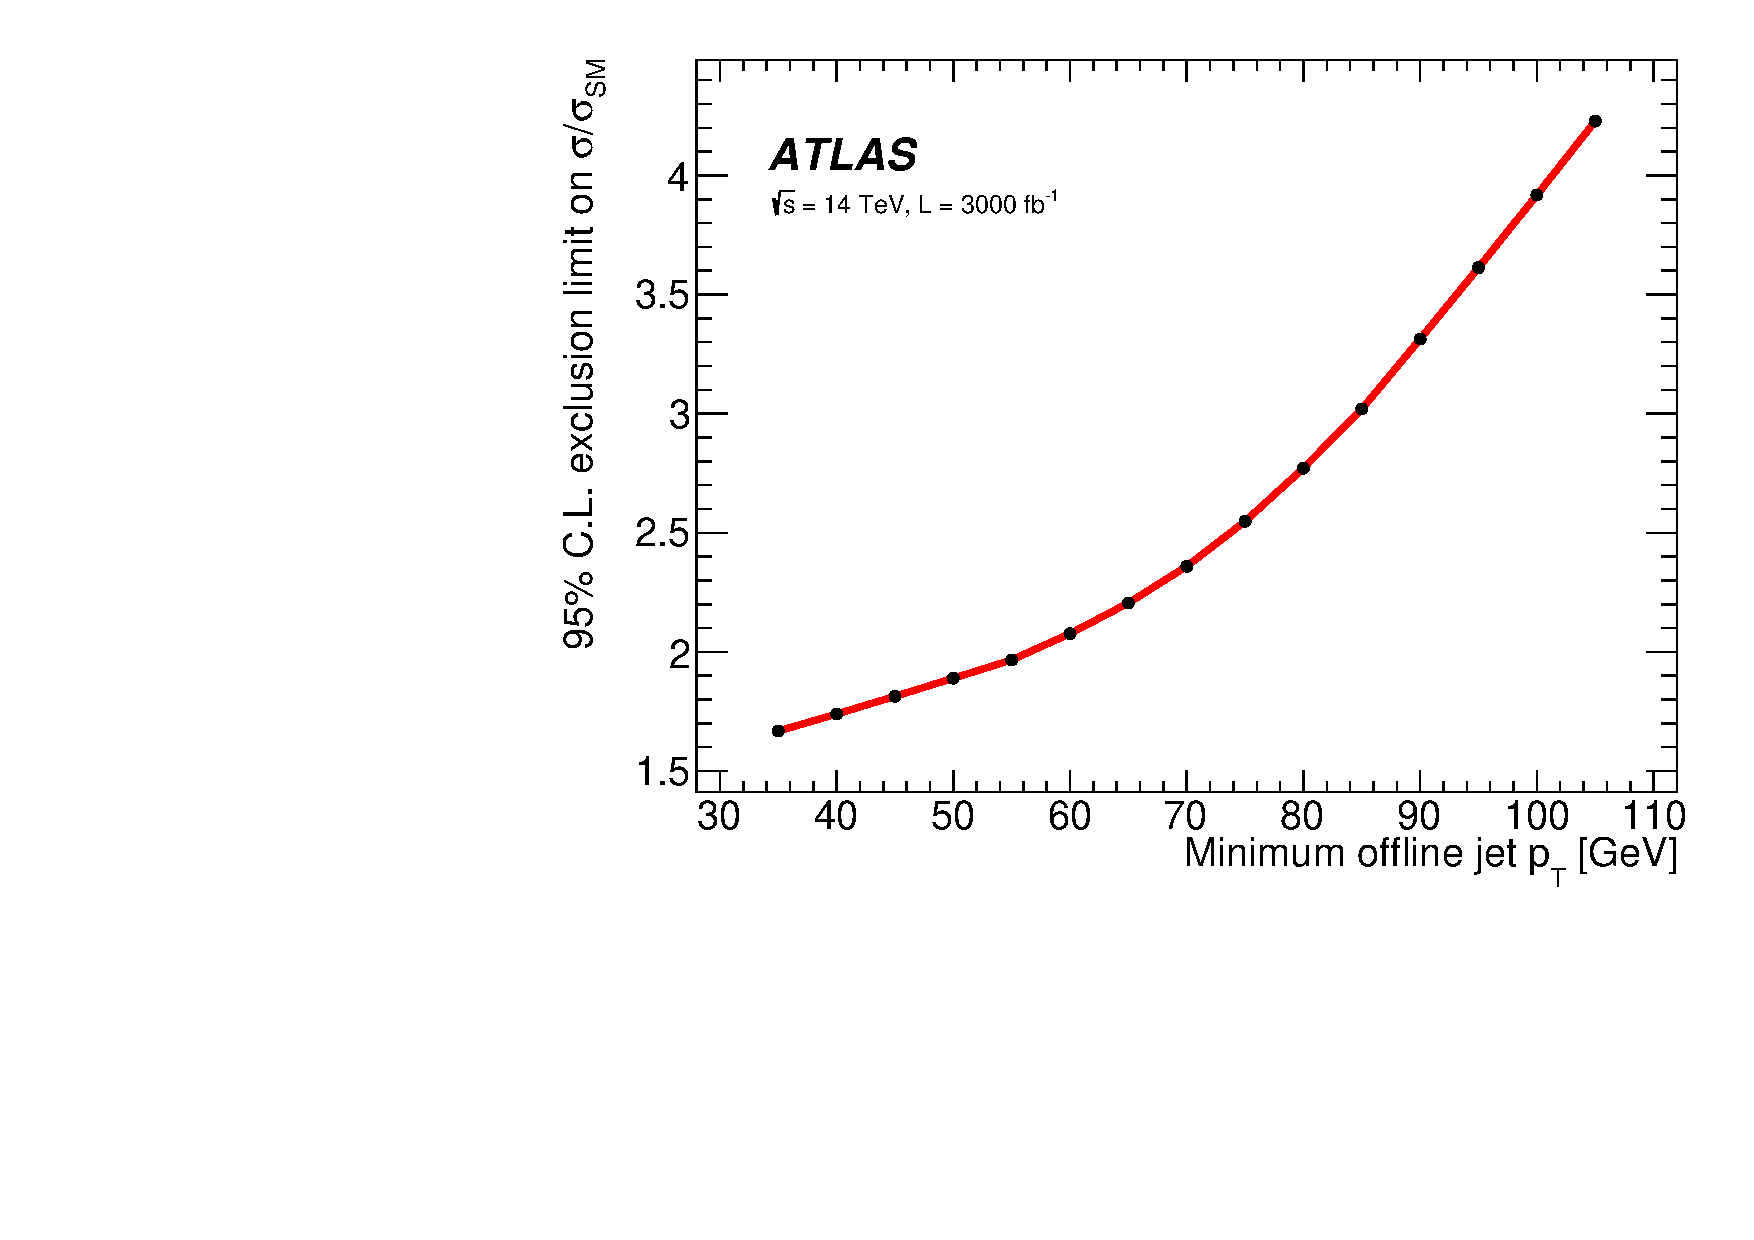
\includegraphics[width=0.75\linewidth]{./figures/future/HL-LHC_jetPt_2016_projections.pdf}
%%   \caption{Expected 95\% C.L. upper limit on the cross-section $\mu\equiv\sigma(\hh\rightarrow\bbbar\bbbar)/\sigma_{\text{SM}}$,
%%     as a function of the online jet $\pt$ threshold \cite{Collaboration:2285584}.}
%%   \label{fig:jetPtExtrapolation}
%%   \end{center}
%% \end{figure}

%% Before analysis improvements can be implemented we must upgrade the ATLAS and CMS detectors such that they can efficiently trigger on $HH$ signal events
%% with all hadronic final states. Figure \ref{fig:jetPtExtrapolation} shows the expected limit on $\mu$ from the $\bbbar\bbbar$ HL-LHC extrapolation \cite{ATL-PHYS-PUB-2016-024}
%% with zero systematic uncertainty as a function of the online jet $\pt$ threshold.
%% Keeping the threshold of a four jet trigger as used in this thesis (Chapter \ref{sec:triggerStudy}) below $\approx60\,\GeV$ will be required to avoid significant losses in
%% sensitivity.

%% The primary trigger used in this thesis requires four jets with transverse momentum above $35\,\GeV$ where at least two jets are \btagged at the 60\% working point.
%% Online \btagging is critical to keeping these \pt thresholds low but, requires high precision tracking for primary and secondary vertex identification.
%% The CPU resources needed for precision tracking grows nonlinearly with the number of pileup interactions and a new approach will be needed in the High Luminosity era
%% with pileup expected to exceed 200 interactions per bunch crossing.

%% The ATLAS collaboration is addressing this issue by developing hardware based track reconstruction systems starting with the Fast TracKer (FTK).
%% The FTK is being integrated with the ATLAS trigger system now and is planned to be used for physics in Run-3 where we expect around 80 pileup interactions per bunch crossing.
%% The FTK is designed to provide track reconstruction for the full inner detector (ID, see Chapter \ref{sec:tracking}) at the 100\,kHz L1 output rate.
%% Software triggers in the HLT can then directly use tracks provided by FTK or use them to seed the full offline tracking algorithm. In either case, the track reconstruction
%% burden placed on the HLT by \bjet triggers will be largely eliminated.

%% The FTK uses a staged, massively parallel architecture with seven types of custom printed circuit boards (PCBs) shown in Figure \ref{fig:ftkDiagram}
%% and hundreds of high speed fiber optic links connecting them.
%% The data flow and staged track fitting process is summarized below:
%% \begin{enumerate}
%%   \item Raw hit data from the ID is clustered in the Input Mezzanine cards (IM).
%%   \item Cluster coordinates and widths are grouped and distributed between Data Formatter boards before being routed to the appropriate track fitting boards.
%%     Clusters from 5 SCT layers and three pixel layers are sent to the first stage tracking boards (AUX) while the data from the other three SCT layers and IBL
%%     are sent to the Second Stage Boards (SSB).
%%   \item The clusters from the eight layers sent to the AUX are converted to coarse resolution hits called Super Strips (SSID). The full resolution clusters are stored
%%     in a linked memory structure by their SSID while the SSIDs are sent to the Associative Memory Board (AMB).
%%   \item The AMB routes the SSID streams through custom ASICs which each store rough track patterns called Roads. The ID number for Roads matched to at least seven
%%     out of eight layers are then sent back to the AUX.
%%   \item The AUX looks up the SSIDs contained in each returned Road and retrieves the corresponding full resolution cluster data. A linearized track candidate $\chi^2$
%%     (goodness of fit) is computed for all possible combinations of clusters in a Road. Track candidates passing a maximum $\chi^2$ threshold are passed on for
%%     overlap removal. The candidate with the lowest $\chi^2$ in a given Road is forwarded to an SSB.
%%   \item The SSB extrapolates the first stage tracks to the other four detector layers and computes a new twelve layer $\chi^2$ and helix parameters.
%%     Overlap removal is then applied to tracks which pass the twelve layer $\chi^2$ threshold.
%%   \item Second stage tracks are formatted by the FTK Level-2 Interface Cards (FLIC) and sent to the Readout System (ROS) for use in the software based triggers.
%% \end{enumerate}

%% \begin{figure}
%%   \begin{center}
%%   \includegraphics[width=\linewidth]{./figures/future/ftkDiagram.pdf}
%%   \caption{The seven custom PCB types of FTK. The full system will consist of 128 Input Mezzanines (IM), 32 Data Formatters (DF), 128 Auxiliary cards (AUX),
%%   128 Associative Memory Boards (AMB), 512 Local AMBs (LAMB), 32 Second Stage Boards (SSB) and 2 FTK Level-2 Interface Cards (FLIC).}
%%   \label{fig:ftkDiagram}
%%   \end{center}
%% \end{figure}



